\documentclass[]{book}

%These tell TeX which packages to use.
\usepackage{array,epsfig}
\usepackage{amsmath}
\usepackage{amsfonts}
\usepackage{amssymb}
\usepackage{amsxtra}
\usepackage{amsthm}
\usepackage{mathrsfs}
\usepackage{color}
\usepackage[margin=2cm,top=2.5cm,headheight=16pt,headsep=0.1in,heightrounded]{geometry}
\usepackage{fancyhdr}
\pagestyle{fancy}
\usepackage{tikz}


%Here I define some theorem styles and shortcut commands for symbols I use often
\theoremstyle{definition}
\newtheorem{defn}{Definition}
\newtheorem{thm}{Theorem}
\newtheorem{cor}{Corollary}
\newtheorem*{rmk}{Remark}
\newtheorem{lem}{Lemma}
\newtheorem*{joke}{Joke}
\newtheorem{ex}{Example}
\newtheorem*{soln}{Solution}
\newtheorem{prop}{Proposition}

\newcommand{\lra}{\longrightarrow}
\newcommand{\ra}{\rightarrow}
\newcommand{\surj}{\twoheadrightarrow}
\newcommand{\graph}{\mathrm{graph}}
\newcommand{\bb}[1]{\mathbb{#1}}
\newcommand{\Z}{\bb{Z}}
\newcommand{\Q}{\bb{Q}}
\newcommand{\R}{\bb{R}}
\newcommand{\C}{\bb{C}}
\newcommand{\N}{\bb{N}}
\newcommand{\M}{\mathbf{M}}
\newcommand{\m}{\mathbf{m}}
\newcommand{\MM}{\mathscr{M}}
\newcommand{\HH}{\mathscr{H}}
\newcommand{\Om}{\Omega}
\newcommand{\Ho}{\in\HH(\Om)}
\newcommand{\bd}{\partial}
\newcommand{\del}{\partial}
\newcommand{\bardel}{\overline\partial}
\newcommand{\textdf}[1]{\textbf{\textsf{#1}}\index{#1}}
\newcommand{\img}{\mathrm{img}}
\newcommand{\ip}[2]{\left\langle{#1},{#2}\right\rangle}
\newcommand{\inter}[1]{\mathrm{int}{#1}}
\newcommand{\exter}[1]{\mathrm{ext}{#1}}
\newcommand{\cl}[1]{\mathrm{cl}{#1}}
\newcommand{\ds}{\displaystyle}
\newcommand{\vol}{\mathrm{vol}}
\newcommand{\cnt}{\mathrm{ct}}
\newcommand{\osc}{\mathrm{osc}}
\newcommand{\LL}{\mathbf{L}}
\newcommand{\UU}{\mathbf{U}}
\newcommand{\support}{\mathrm{support}}
\newcommand{\AND}{\;\wedge\;}
\newcommand{\OR}{\;\vee\;} 
\newcommand{\Oset}{\varnothing}
\newcommand{\st}{\ni}
\newcommand{\wh}{\widehat}
\newcommand{\vect}[1]{\overrightarrow{#1}}

%Pagination stuff.
\setlength{\topmargin}{-.3 in}
%\setlength{\oddsidemargin}{0in}
%\setlength{\evensidemargin}{0in}
\setlength{\textheight}{9.in}
\setlength{\textwidth}{6.5in}
\cfoot{page \thepage}
\lhead{MEU303 - Alg\`ebre}
\rhead{TD1}
\pagestyle{fancy}


\begin{document}

\subsection*{Rappel de cours}
\begin{defn}
Bla bla
\end{defn}



\newpage
\subsection*{Exercice 1}
\subsection*{Exercice 1.a}
Soit $D$ une droite vectoriel, $D=\{M | \vect{OM} = \lambda \vect{v}, \lambda \in \R \}$ et $D'$ une demi-droite ferm\'ee (ou ouverte) d'origine $A'$, $D'=\{M' | \vect{A'M'} = \lambda' \vect{u}, \lambda' \in \R^{+} \}$.

Soit $A$ le point de la droite $D$ tel que $F(\vect{OA}) = \vect{OA'}$, et les 2 points $M_1$ et $M_2$ tel que le point $A$ soit au milieu du segment $M_1M_2$. Donc $\vect{AM_1} = -\vect{AM_2}$.
Si l'application lin\'eaire $F$ existe alors on a $F(\vect{AM_1}) = F(-\vect{AM_2}) = -F(\vect{AM_2})$.  
	
Soit le point $M'_2$ tel que $F(\vect{AM_2}) = \vect{A'M'_2}$. Il existe $\lambda'_2$ tel que $\vect{A'M_2}= \lambda'_2 \vect{u}, \lambda'_2 \in \R^{+}$.  Il n'existe pas de $\lambda_1$ positif tel que $\vect{A'M_1}= \lambda'_1 \vect{u}$. Ceci contredit l'existence de l'application lin\'eaire.

\subsection*{Exercice 1.b}
Si l'application lin\'eaire $F$ existe alors $F(c\vect{O}) = cF(\vect{O})$, mais par d\'efinition de $O$ on a $c\vect{O} = \vect{O}$ donc 
$$
F(c\vect{O}) = F(\vect{O}) = cF(\vect{O})
$$

Donc $F(\vect{O}) = \vect{O}$ car $c$ est diff\'erent de 0. Ceci contredit l'hypoth\`ese que l'image de l'application $F$ est priv\'ee de l'origine $O$.

\subsection*{Exercice 1.c}
Soit l'application $F: \R^2 \setminus{O} \to \R$ tel que $F(x,y) = x-y$. Montrons que l'application $F$ est lin\'eaire.
$$
F(c(x,y)) = F((cx, cy)) = cx-cy = c(x-y) = cF((x,y))
$$
et 
$$
F(A_1) + F(A_2) = F(x_1, y_1) + F(x_2, y_2) = x_1-y_1+x_2-y_2 = (x_1+x_2)-(y_1+y_2) = F((x_1+x_2, y_1+y_2)) = F(A_1+A_2)
$$


\subsection*{Exercice 2}
\subsection*{Exercice 2.a}
\begin{center}
\begin{tikzpicture}
	\draw[thin,gray!40] (-5,-5) grid (5,5);
	\draw[<->] (-5,0)--(5,0) node[right]{$x$};
	\draw[<->] (0,-5)--(0,5) node[above]{$y$};
	
    \draw[->, ultra thick, green,  arrows={-latex}]  (0,0) -- (0,1) node[sloped,midway,above=-0.1cm] {$\mathsf{e'_1}$};
    \draw[->, ultra thick, green,  arrows={-latex}]  (0,0) -- (0,-2) node[sloped,midway,above=-0.1cm] {$\mathsf{e'_2}$};
    \draw[->, ultra thick, green,  arrows={-latex}]  (0,0) -- (2,-4) node[sloped,midway,above=-0.1cm] {$\mathsf{e'_3}$};

    \draw[->, ultra thick, blue,  arrows={-latex}]  (0,0) -- (1,0) node[sloped,midway,above=-0.1cm] {$\mathsf{e_1}$};
    \draw[->, ultra thick, blue,  arrows={-latex}]  (0,0) -- (3,2) node[sloped,midway,above=-0.1cm] {$\mathsf{e_2}$};
    \draw[->, ultra thick, blue,  arrows={-latex}]  (0,0) -- (1,-2) node[sloped,midway,above=-0.1cm] {$\mathsf{e_3}$};
\end{tikzpicture}
\end{center}

$F(e_2) = F(-e_3 + 4e_1) = -F(e_3) + 4F(e_1) = -e'_3 +4e'_1 = -(2,-4) + 4(0,1) = (-2,0) \neq e'_2 = (3,2)$, donc pas lin\'eaire.  




\subsection*{Exercice 2.b}
$$
\left\{
\begin{array}{l l}
(1, 0, 0) . 
\begin{pmatrix}
m_{11} & m_{21} & m_{31} \\
m_{12} & m_{22} & m_{32} \\
m_{13} & m_{23} & m_{33}
\end{pmatrix} 
& = (0, 0 ,0) \\
 
(0, 1, 0) . 
\begin{pmatrix}
m_{11} & m_{21} & m_{31} \\
m_{12} & m_{22} & m_{32} \\
m_{13} & m_{23} & m_{33}
\end{pmatrix}
& = (0, 0 ,1) \\

(0, 0, 1) . 
\begin{pmatrix}
m_{11} & m_{21} & m_{31} \\
m_{12} & m_{22} & m_{32} \\
m_{13} & m_{23} & m_{33}
\end{pmatrix}
& = (1, 0 ,0) \\
\end{array}
\right.
$$ 

donc
$$
\left\{
\begin{array}{l l}
m_{11} & = 0 \\
m_{21} & = 0 \\
m_{31} & = 0 \\
m_{12} & = 0 \\
m_{22} & = 0 \\
m_{32} & = 1 \\
m_{13} & = 1 \\
m_{23} & = 0 \\
m_{33} & = 0 \\
\end{array}
\right.
$$


Solution unique.
$$
(x, y, z) .
\begin{pmatrix}
0 & 0 & 0 \\
0 & 0 & 1 \\
1 & 0 & 0 \\
\end{pmatrix}
=
(z, 0, y)
$$

\subsection*{Exercice 2.c}
$$
\left\{
\begin{array}{l l}
(1, 0, 0) . 
\begin{pmatrix}
m_{11} & m_{21} & m_{31} & m_{41} \\
m_{12} & m_{22} & m_{32} & m_{42} \\
m_{13} & m_{23} & m_{33} & m_{43} \\
\end{pmatrix} 
& = (1,0,0,0) (\text{ie } X^3) \\
 
(0, 1, 0) . 
\begin{pmatrix}
m_{11} & m_{21} & m_{31} & m_{41} \\
m_{12} & m_{22} & m_{32} & m_{42} \\
m_{13} & m_{23} & m_{33} & m_{43} \\
\end{pmatrix}
& = (0, 1, 0, 0) (\text{ie } X^2)\\

(0, 0, 1) . 
\begin{pmatrix}
m_{11} & m_{21} & m_{31} & m_{41} \\
m_{12} & m_{22} & m_{32} & m_{42} \\
m_{13} & m_{23} & m_{33} & m_{43} \\
\end{pmatrix}
& = (0, 0, 1, 0) (\text{ie } X)\\

(1, 1, 1) . 
\begin{pmatrix}
m_{11} & m_{21} & m_{31} & m_{41} \\
m_{12} & m_{22} & m_{32} & m_{42} \\
m_{13} & m_{23} & m_{33} & m_{43} \\
\end{pmatrix}
& = (0, 0, 0, 1) (\text{ie } 1)\\

\end{array}
\right.
$$ 

donc
$$
\left\{
\begin{array}{l l}
m_{11} & = 1 \\
m_{21} & = 0 \\
m_{31} & = 0 \\
m_{41} & = 0 \\
m_{12} & = 0 \\
m_{22} & = 1 \\
m_{32} & = 0 \\
m_{42} & = 0 \\
m_{13} & = 0 \\
m_{23} & = 0 \\
m_{33} & = 1 \\
m_{43} & = 0 \\
m_{11} + m_{12} + m_{13} & = 0 \\
m_{21} + m_{22} + m_{23} & = 0 \\
m_{31} + m_{32} + m_{33} & = 0 \\
m_{41} + m_{42} + m_{43} & = 1 \\
\end{array}
\right.
$$

Pas de solution.
QED

\subsection*{Exercice 2.d}
$$
\left\{
\begin{array}{l l}
(1, 0, 0, 0, 1) . 
\begin{pmatrix}
m_{11} & m_{21} \\
m_{12} & m_{22} \\
m_{13} & m_{23} \\
m_{14} & m_{24} \\
m_{15} & m_{25} \\
\end{pmatrix} 
& = (2, -1) \\

(0, 0, 1, 0, 0) . 
\begin{pmatrix}
m_{11} & m_{21} \\
m_{12} & m_{22} \\
m_{13} & m_{23} \\
m_{14} & m_{24} \\
m_{15} & m_{25} \\
\end{pmatrix} 
& = (3, 0) \\
\end{array}
\right.
$$

donc
$$
\left\{
\begin{array}{l l}
m_{11} + m_{15} & = 2 \\
m_{21} + m_{25} & = -1 \\
m_{13} & = 3 \\
m_{23} & = 0 \\
\end{array}
\right.
$$

Il y a un infinit\'e d'applications:
$$
(X^3, X^2, X, 1) .
\begin{pmatrix}
m_{11} & m_{21} \\
m_{12} & m_{22} \\
3 & 0 \\
m_{14} & m_{24} \\
2 - m_{11} & -1 - m_{21} \\
\end{pmatrix} 
=
(m_{11}X^4+m_{12}X^3+3X^2+m_{14}X+ 2 - m_{11}, m_{21}X^4+m_{22}X^3+m_{24}X - 1- m_{21})
$$

\subsection*{Exercice 2.e}
$$
\left\{
\begin{array}{l l}
(0, 0, 2, 1) . 
\begin{pmatrix}
m_{11} & m_{21} & m_{31} \\
m_{12} & m_{22} & m_{32} \\
m_{13} & m_{23} & m_{33} \\
m_{14} & m_{24} & m_{34} \\
\end{pmatrix} 
& = (0, 1, 1) \\

(1, 1, 1, 0) . 
\begin{pmatrix}
m_{11} & m_{21} & m_{31} \\
m_{12} & m_{22} & m_{32} \\
m_{13} & m_{23} & m_{33} \\
m_{14} & m_{24} & m_{34} \\
\end{pmatrix} 
& = (0, 2, 2) \\

(2, 2, 0, 1) . 
\begin{pmatrix}
m_{11} & m_{21} & m_{31} \\
m_{12} & m_{22} & m_{32} \\
m_{13} & m_{23} & m_{33} \\
m_{14} & m_{24} & m_{34} \\
\end{pmatrix} 
& = (0, 3, 3) \\
\end{array}
\right.
$$

donc
$$
\left\{
\begin{array}{l l l}
2m_{13} + m_{14} & = 0 & \to m_{14} = -2m_{13} \\
2m_{23} + m_{24} & = 1 & \to m_{24} = 1-2m_{13} \\
2m_{33} + m_{34} & = 1 & \to m_{34} = 1-2m_{33} \\
m_{11} + m_{12} + m_{13} & = 0 & \\
m_{21} + m_{22} + m_{23} & = 2 & \\
m_{31} + m_{32} + m_{33} & = 2 & \\
2m_{11} + 2m_{12} + m_{14} & = 0 & \to 2m_{11} + 2m_{12} - 2m_{13} = 0 \\
2m_{21} + 2m_{22} + m_{24} & = 3 & \to 2m_{21} + 2m_{22} - 2m_{23} = 2 \\
2m_{31} + 2m_{32} + m_{34} & = 3 & \to 2m_{31} + 2m_{32} - 2m_{33} = 2 \\
\end{array}
\right.
$$

Il y a un infinit\'e d'applications:
$$
\begin{pmatrix}
m_{11} & m_{21} & m_{31} \\
-m_{11} & 3/2-m_{21} & 3/2-m_{31} \\
0 & 1/2 & 1/2 \\
0 & 0 & 0 \\
\end{pmatrix} 
$$

\subsection*{Exercice 2.f}
??

\subsection*{Exercice 3}
\subsection*{Exercice 3.a}
\begin{center}
\begin{tikzpicture}
	\draw[thin,gray!40] (-4,-4) grid (4,4);
	\draw[<->] (-4,0)--(4,0) node[right]{$x$};
	\draw[<->] (0,-4)--(0,4) node[above]{$y$};
	
    \draw[->, ultra thick, blue,  arrows={-latex}]  (0,0) -- (1,0) node[sloped,midway,above=-0.1cm] {$\mathsf{e_1}$};
    \draw[->, ultra thick, blue,  arrows={-latex}]  (0,0) -- (0,1) node[sloped,midway,above=-0.1cm] {$\mathsf{e_2}$};
    \draw[->, ultra thick, blue,  arrows={-latex}]  (0,0) -- (2,0) node[sloped,midway,above=-0.1cm] {$\mathsf{v_1}$};
    \draw[->, ultra thick, blue,  arrows={-latex}]  (0,0) -- (2,1) node[sloped,midway,above=-0.1cm] {$\mathsf{v_2}$};

    \draw[->, ultra thick, green,  arrows={-latex}]  (0,0) -- (1,1) node[sloped,midway,above=-0.1cm] {$\mathsf{e'_1}$};
    \draw[->, ultra thick, green,  arrows={-latex}]  (0,0) -- (-1,1) node[sloped,midway,above=-0.1cm] {$\mathsf{e'_2}$};
    \draw[->, ultra thick, green,  arrows={-latex}]  (0,0) -- (2,2) node[sloped,midway,above=-0.1cm] {$\mathsf{v'_1}$};
    \draw[->, ultra thick, green,  arrows={-latex}]  (0,0) -- (1,3) node[sloped,midway,above=-0.1cm] {$\mathsf{v'_2}$};
\end{tikzpicture}
\end{center}

On a $F(v_1) = F(2e_1) = 2F(e_1) = (2,2)$ et $F(v_2) = F(2e_1+e_2) = 2F(e_1)+F(e_2) = (1,3)$

$$
F = 
\begin{pmatrix}
1 & 1 \\
-1 & 1 \\
\end{pmatrix} 
$$

$F$ est ????


\subsection*{Exercice 3.b}
\begin{center}
\begin{tikzpicture}
	\draw[thin,gray!40] (-5,-5) grid (5,5);
	
	\draw[<->] (-5,0)--(5,0) node[right]{$x$};
	\draw[<->] (0,-5)--(0,5) node[above]{$y$};
	
    \draw[->, ultra thick, blue,  arrows={-latex}]  (0,0) -- (1,1) node[sloped,midway,above=-0.1cm] {$\mathsf{e_1}$};
    \draw[->, ultra thick, blue,  arrows={-latex}]  (0,0) -- (0,1) node[sloped,midway,above=-0.1cm] {$\mathsf{e_2}$};
    \draw[->, ultra thick, blue,  arrows={-latex}]  (0,0) -- (1,0) node[sloped,midway,above=-0.1cm] {$\mathsf{v_1}$};
    \draw[->, ultra thick, blue,  arrows={-latex}]  (0,0) -- (2,-1) node[sloped,midway,above=-0.1cm] {$\mathsf{v_2}$};

    \draw[->, ultra thick, green,  arrows={-latex}]  (0,0) -- (4,1) node[sloped,midway,above=-0.1cm] {$\mathsf{e'_1}$};
    \draw[->, ultra thick, green,  arrows={-latex}]  (0,0) -- (3,1) node[sloped,midway,above=-0.1cm] {$\mathsf{e'_2}$};
    \draw[->, ultra thick, green,  arrows={-latex}]  (0,0) -- (1,0) node[sloped,midway,above=-0.1cm] {$\mathsf{v'_1}$};
    \draw[->, ultra thick, green,  arrows={-latex}]  (0,0) -- (-1,-1) node[sloped,midway,above=-0.1cm] {$\mathsf{v'_2}$};
\end{tikzpicture}
\end{center}

On a $F(v_1) = F(e_1-e_2) = F(e_1) - F(e_2) = (1,0)$ et $F(v_2) = F(2e_1-3e_2) = 2F(e_1)-3F(e_2) = (-1,-1)$

$$
F = 
\begin{pmatrix}
1 & 0 \\
3 & 1 \\
\end{pmatrix} 
$$

$F$ est ??.

\subsection*{Exercice 3.c}
\begin{center}
\begin{tikzpicture}
	\draw[thin,gray!40] (-5,-5) grid (5,5);
	
	\draw[<->] (-5,0)--(5,0) node[right]{$x$};
	\draw[<->] (0,-5)--(0,5) node[above]{$y$};
	
    \draw[->, ultra thick, blue,  arrows={-latex}]  (0,0) -- (3,3) node[sloped,midway,above=-0.1cm] {$\mathsf{e_1}$};
    \draw[->, ultra thick, blue,  arrows={-latex}]  (0,0) -- (0,-3) node[sloped,midway,above=-0.1cm] {$\mathsf{e_2}$};
    \draw[->, ultra thick, blue,  arrows={-latex}]  (0,0) -- (1,2) node[sloped,midway,above=-0.1cm] {$\mathsf{v_1}$};
    \draw[->, ultra thick, blue,  arrows={-latex}]  (0,0) -- (2,1) node[sloped,midway,above=-0.1cm] {$\mathsf{v_2}$};

    \draw[->, ultra thick, green,  arrows={-latex}]  (0,0) -- (1,2) node[sloped,midway,above=-0.1cm] {$\mathsf{e'_1}$};
    \draw[->, ultra thick, green,  arrows={-latex}]  (0,0) -- (-2,-4) node[sloped,midway,above=-0.1cm] {$\mathsf{e'_2}$};
    \draw[->, ultra thick, green,  arrows={-latex}]  (0,0) -- (2.333,4.666) node[sloped,midway,above=-0.1cm] {$\mathsf{v'_1}$};
    \draw[->, ultra thick, green,  arrows={-latex}]  (0,0) -- (0,0) node[sloped,midway,above=-0.1cm] {$\mathsf{v'_2}$};
\end{tikzpicture}
\end{center}

On a $F(v_1) = F(1/3e_1-e_2) = 1/3F(e_1) - F(e_2) = (7/3,14/3)$ et $F(v_2) = F(2/3e_1+1/3e_2) = 2/3F(e_1)+1/3F(e_2) = (0,0)$

$$
F = 
\begin{pmatrix}
7 & -2/3 \\
-2 & 4/3 \\
\end{pmatrix} 
$$

$F$ est projection sur la droite $y=2x$ suivant le vecteur $(-2,-1)$.


\end{document}

